\chapter{空气，一种混合气体}\label{ch:g4:air-a-mixture-of-gases}

在风大的日子里，风筝拉扯着它的线，
湖面上，帆鼓起来，推着小船前进。推动它们的东西，
我们却看不见。那就是\omterm{def:g4:air-a-mixture-of-gases:air}{空气}。我们看不见\omterm{def:g4:air-a-mixture-of-gases:air}{空气}，
但它无处不在，充满每一个空瓶和每一间屋子，
我们每一次呼吸都会吸入它。\omterm{def:g4:air-a-mixture-of-gases:air}{空气}是由什么组成的？

\begin{recall}
\omterm{def:g2:mixing-and-dissolving:mix}{混合}就是把不同的东西放在一起；得到的是这些东西的
\omterm{def:g2:mixing-and-dissolving:mix}{混合}物，\omterm{def:g2:mixing-and-dissolving:mix}{混合}时没有任何物质损失
（见\cref{ch:g2:mixing-and-dissolving}）。
\end{recall}

\begin{omfigure}
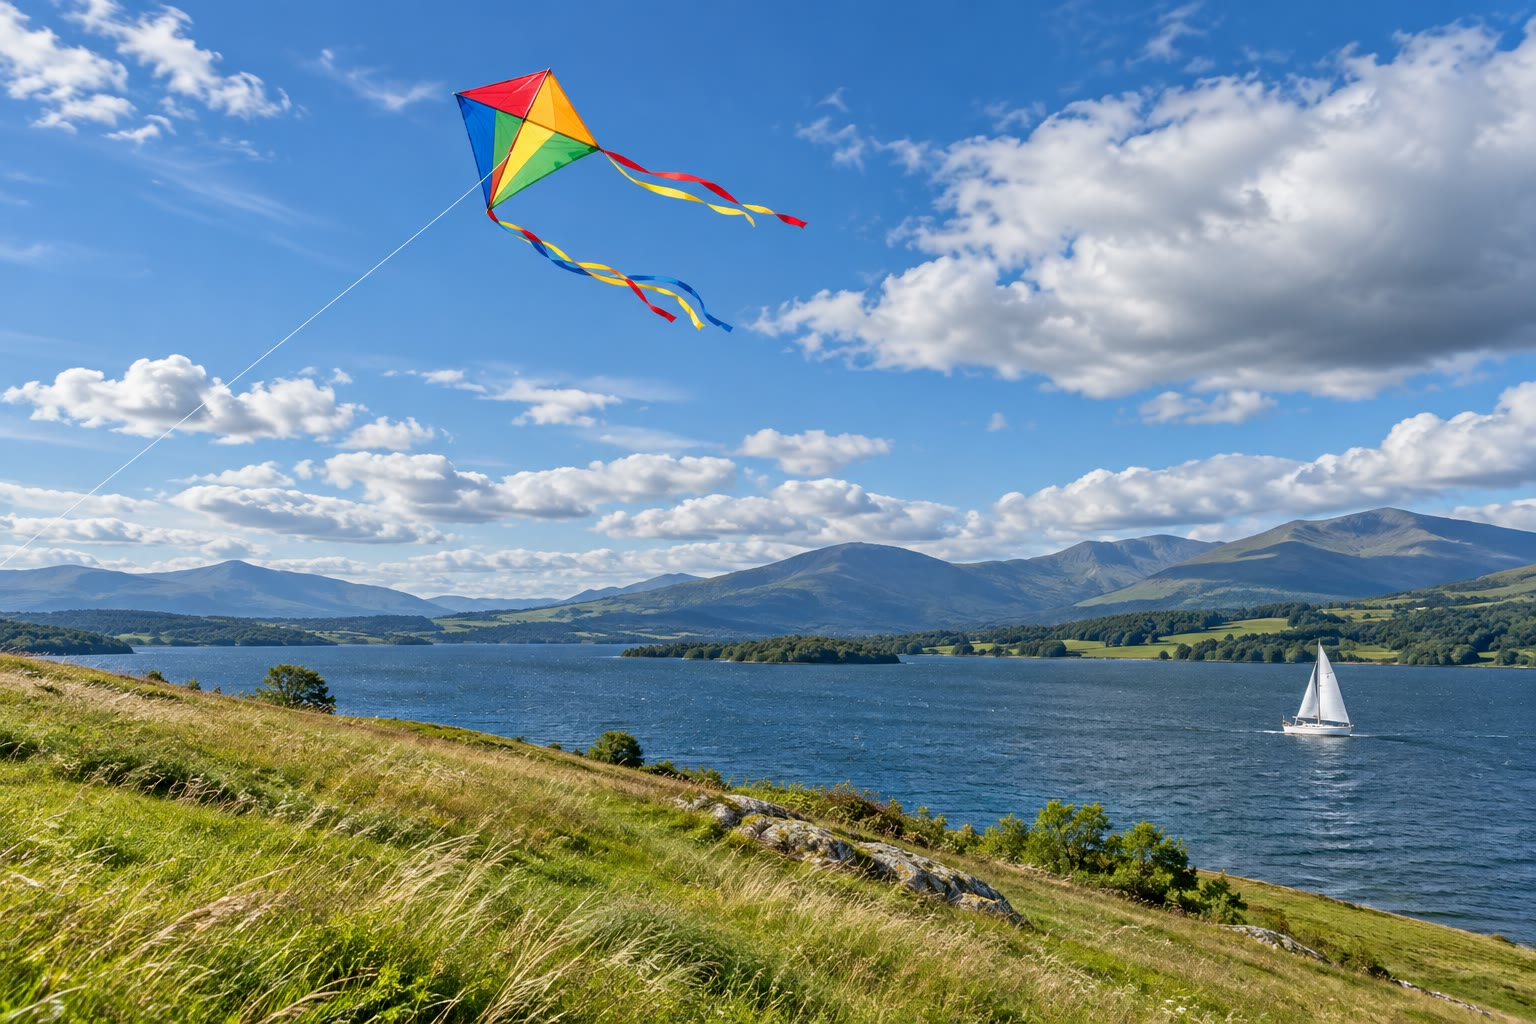
\includegraphics[width=0.6\linewidth]{images/book1/ai/g4-kite-day.jpg}

{\small 风筝与帆：\omterm{def:g4:air-a-mixture-of-gases:air}{空气}看不见，但它能推动物体。}
\end{omfigure}

\section{空气无处不在}

\begin{example}[倒扣的玻璃杯]\label{ex:g4:air-a-mixture-of-gases:glass}
一张干燥的纸巾被塞到空玻璃杯的底部。玻璃杯
被倒扣过来，竖直压入一碗水中。
拿出来时，纸巾仍是干的。这个玻璃杯并非
空的：杯中充满了\omterm{def:g4:air-a-mixture-of-gases:air}{空气}，\omterm{def:g4:air-a-mixture-of-gases:air}{空气}把水挡在了外面。
\end{example}

\begin{omfigure}
\begin{tikzpicture}[font=\small, scale=1.3]
  \pic[transform shape] at (0,0) {trough};
  % the upturned glass, rim at y = 0.35, base at y = 2.35
  \fill[white] (-0.8,0.5) rectangle (0.8,0.95);
  \pic[transform shape, rotate=180] at (0,2.35) {beaker={0}{white}};
  % the tissue at the top, inside
  \fill[white, draw=black!45, rounded corners=1.5pt] (-0.4,2.33) -- (-0.3,2.05)
    -- (-0.1,2.12) -- (0.05,1.98) -- (0.25,2.1) -- (0.42,2.02) -- (0.45,2.33) -- cycle;
  \draw[<-, omProp, thick] (0.45,2.12) -- (2.4,2.5) node[right, text=black]
    {一张干燥的纸巾};
  \draw[<-, omProp, thick] (0.3,1.2) -- (2.4,1.4) node[right, text=black]
    {空气：把水挡在外面};
  \draw[<-, omProp, thick] (1.4,0.7) -- (2.4,0.55) node[right, text=black]
    {水};
\end{tikzpicture}

{\small 玻璃杯倒扣着压入水中。被困在杯内的\omterm{def:g4:air-a-mixture-of-gases:air}{空气}
把水挡在外面，纸巾保持干燥。}
\end{omfigure}


\begin{remark}[空气是一种气体]\label{rem:g4:air-a-mixture-of-gases:gas}
\omterm{def:g4:air-a-mixture-of-gases:air}{空气}是一种气体：它没有固定的形状，会扩散开来充满任何
容器。它同样是物质，充满\omterm{def:g4:air-a-mixture-of-gases:air}{空气}的气球
比空着的同一只气球略重一些。气体是什么，以及它们为何
这样表现，在物理分册中有讲述。
\end{remark}

\section{空气是混合物}

\begin{definition}[空气]\label{def:g4:air-a-mixture-of-gases:air}
\emph{空气}\index{空气}是包围地球的\omterm{def:g2:mixing-and-dissolving:mix}{混合}气体。
它不是单一的气体：其中混有若干种气体，
它们可以彼此分离。
\end{definition}

\begin{proposition}[空气的组成]\label{prop:g4:air-a-mixture-of-gases:composition}
% ledger: air:N2, air:O2, air:Ar, air:trace, air:CO2, air:H2O
不计水蒸气，\omterm{def:g4:air-a-mixture-of-gases:air}{空气}由下列成分组成：
\begin{itemize}
  \item \textbf{氮气}，约占\omterm{def:g4:air-a-mixture-of-gases:air}{空气}的五分之四；
  \item \textbf{氧气}，约占\omterm{def:g4:air-a-mixture-of-gases:air}{空气}的五分之一；
  \item 少量\textbf{氩气}，约占 100 份中的 1 份；
  \item 极少量的\textbf{二氧化碳}，约占 10\,000 份中的 4 份，
        以及微量的其他气体。
\end{itemize}
\omterm{def:g4:air-a-mixture-of-gases:air}{空气}中还含有\textbf{水蒸气}，它看不见：干燥寒冷的日子里含量很少，
炎热潮湿的日子里可达约 100 份中的 4 份。
\end{proposition}

\begin{example}[一百瓶空气]\label{ex:g4:air-a-mixture-of-gases:hundred}
% ledger: air:N2, air:O2, air:Ar
想象有 100 瓶干燥的\omterm{def:g4:air-a-mixture-of-gases:air}{空气}，把\omterm{def:g4:air-a-mixture-of-gases:air}{空气}中的气体
分别装入不同的瓶中。约 78 瓶装氮气，21 瓶装氧气，
最后一瓶装氩气，还有只够几滴的二氧化碳，
以及其他气体。
\end{example}

\begin{omfigure}
\begin{tikzpicture}[font=\small, x=0.42cm, y=0.42cm]
  \foreach \k in {0,...,99} {
    \pgfmathtruncatemacro\col{mod(\k,10)}
    \pgfmathtruncatemacro\row{9-int(\k/10)}
    \ifnum\k<78 \def\c{omDef!45}\else\ifnum\k<99 \def\c{red!45}\else\def\c{cyan!60}\fi\fi
    \fill[\c, draw=white, line width=0.8pt] (\col,\row) rectangle ++(1,1);
  }
  \fill[omDef!45] (12,8) rectangle ++(1,1);
  \node[anchor=west] at (13.3,8.5) {氮气：78 格};
  \fill[red!45] (12,6) rectangle ++(1,1);
  \node[anchor=west] at (13.3,6.5) {氧气：21 格};
  \fill[cyan!60] (12,4) rectangle ++(1,1);
  \node[anchor=west, align=left] at (13.3,4.5) {氩气、二氧化碳 \\ 及其余气体：1 格};
\end{tikzpicture}

{\small 一百格干燥\omterm{def:g4:air-a-mixture-of-gases:air}{空气}。右下角的一格
装的是氩气，以及小到无法单独画出的二氧化碳。}
\end{omfigure}

\begin{remark}[气体的名称]\label{rem:g4:air-a-mixture-of-gases:names}
氮气、氧气、氩气和二氧化碳都是气体的名称。
它们都是无色的，没有气味。后面的章节将说明
它们各自由什么构成，直到构成一切物质的微小粒子。
\end{remark}

\section{我们吸入和呼出的空气}

\begin{proposition}[呼出的空气]\label{prop:g4:air-a-mixture-of-gases:breath}
% ledger: breath:O2, breath:CO2, breath:N2, air:O2, air:CO2
我们呼出的\omterm{def:g4:air-a-mixture-of-gases:air}{空气}并不是吸入的\omterm{def:g4:air-a-mixture-of-gases:air}{空气}。人体会
吸收一部分氧气，并排出二氧化碳和水蒸气：
\begin{itemize}
  \item 吸入的\omterm{def:g4:air-a-mixture-of-gases:air}{空气}中，氧气约占每 100 份中的 21 份，而
        呼出的\omterm{def:g4:air-a-mixture-of-gases:air}{空气}中仅约占每 100 份中的 16 份；
  \item 二氧化碳的含量由约 10\,000 份中的 4 份，
        增至约每 100 份中的 4 份，约为原来的一百倍；
  \item 氮气呼出时的含量与吸入时相同。
\end{itemize}
\end{proposition}

\begin{omfigure}
\begin{tikzpicture}
\begin{axis}[ybar, width=0.8\linewidth, height=5.2cm, bar width=12pt,
    ymin=0, ymax=90, ylabel={每 100 份中},
    symbolic x coords={nitrogen, oxygen, carbon dioxide}, xtick=data, xticklabels={氮气, 氧气, 二氧化碳},
    tick label style={font=\small}, label style={font=\small},
    xticklabel style={text height=1.6ex, text depth=0.4ex},
    legend style={font=\small, at={(0.98,0.95)}, anchor=north east},
    nodes near coords, nodes near coords style={font=\footnotesize},
    enlarge x limits=0.25, axis lines*=left, ymajorgrids,
    grid style={gray!20}]
% ledger: air:N2, air:O2, air:CO2, breath:N2, breath:O2, breath:CO2 (rounded)
\addplot[fill=omDef!45, draw=omDef] coordinates
  {(nitrogen,78) (oxygen,21) (carbon dioxide,0)};
\addplot[fill=omProp!55, draw=omProp] coordinates
  {(nitrogen,78) (oxygen,16) (carbon dioxide,4)};
\legend{吸入, 呼出}
\end{axis}
\end{tikzpicture}

{\small 吸入与呼出的\omterm{def:g4:air-a-mixture-of-gases:air}{空气}，按每 100 份计（未计水蒸气，
数字已取整）。吸入\omterm{def:g4:air-a-mixture-of-gases:air}{空气}中的二氧化碳为 10\,000 份中的 4 份，
太少，无法画成柱形。}
\end{omfigure}

\begin{example}[拥挤的教室]\label{ex:g4:air-a-mixture-of-gases:room}
在一间关着窗户的小教室里，三十个人整个上午都在呼出
二氧化碳。教室里的\omterm{def:g4:air-a-mixture-of-gases:air}{空气}含氧量渐渐减少，二氧化碳渐渐增多，
人们便感到疲倦。打开
窗户，新鲜\omterm{def:g4:air-a-mixture-of-gases:air}{空气}便重新进入。
\end{example}

\begin{omfigure}
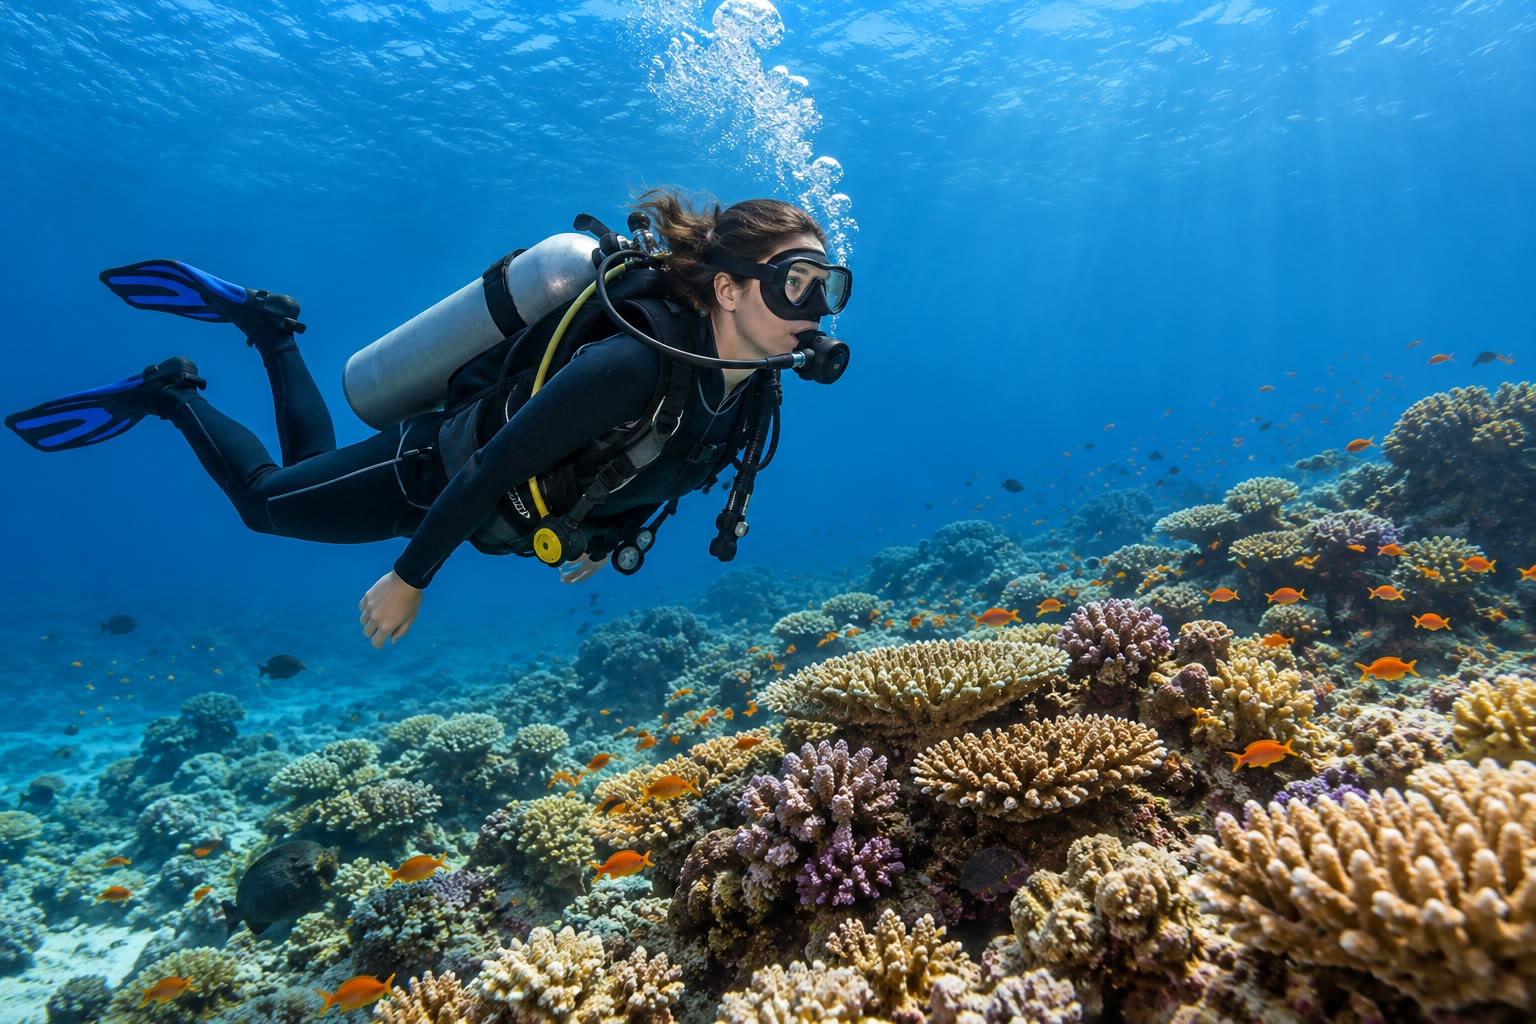
\includegraphics[width=0.55\linewidth]{images/book1/ai/g4-scuba-diver.jpg}

{\small 潜水员用背上气瓶中的\omterm{def:g4:air-a-mixture-of-gases:air}{空气}呼吸；水中的
气泡就是呼出的\omterm{def:g4:air-a-mixture-of-gases:air}{空气}。}
\end{omfigure}

\begin{remark}[潜水员为何呼吸空气]\label{rem:g4:air-a-mixture-of-gases:diver}
潜水员的气瓶里装的是压缩进小空间的\omterm{def:g4:air-a-mixture-of-gases:air}{空气}，而
不是纯氧：在深水下呼吸纯氧是危险的。\omterm{def:g4:air-a-mixture-of-gases:air}{空气}中的
氮气用来稀释氧气。
\end{remark}

\section{生命与燃烧所需的氧气}

\begin{proposition}[氧气会被生物和火焰消耗]\label{prop:g4:air-a-mixture-of-gases:oxygen}
在\omterm{def:g4:air-a-mixture-of-gases:air}{空气}的所有气体中，生物和火焰所需要的
正是氧气。人和动物呼吸时吸入氧气，火焰则
从周围的\omterm{def:g4:air-a-mixture-of-gases:air}{空气}中获取氧气。绿色植物在白天
会将氧气释放回\omterm{def:g4:air-a-mixture-of-gases:air}{空气}中。
\end{proposition}

\begin{inthelab}[广口瓶下的蜡烛]
教师将一支蜡烛放在一块瓷砖上点燃，再把一个大玻璃
广口瓶缓缓罩在蜡烛上。火焰变小、闪烁，几
秒后熄灭：火焰周围的\omterm{def:g4:air-a-mixture-of-gases:air}{空气}含氧太少，无法维持
燃烧。若改用容积两倍大的广口瓶罩住，蜡烛
大约能多烧一倍的时间，因为瓶中\omterm{def:g4:air-a-mixture-of-gases:air}{空气}约为两倍，
氧气也约为两倍，可供消耗。
\end{inthelab}

\begin{omfigure}
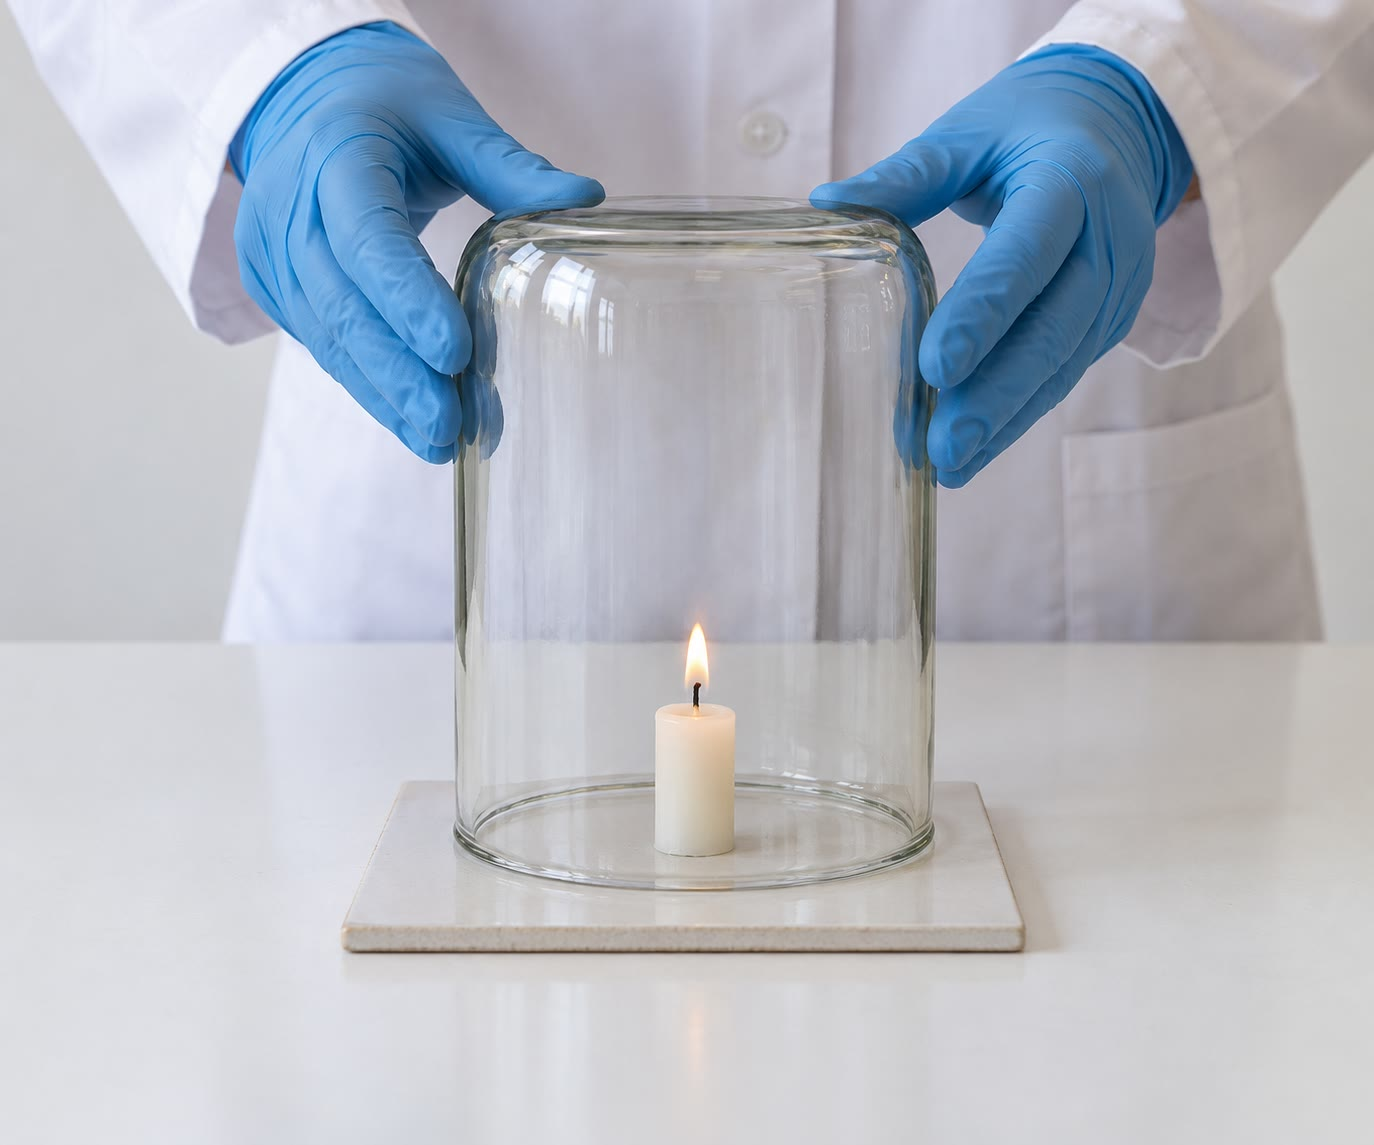
\includegraphics[width=0.5\linewidth]{images/book1/ai/g4-candle-jar-lab.jpg}

{\small 罩在玻璃广口瓶下的蜡烛，火焰周围的
氧气太少时便会熄灭。}
\end{omfigure}

\begin{remark}[氮气不能燃烧]\label{rem:g4:air-a-mixture-of-gases:nitrogen}
氮气是\omterm{def:g4:air-a-mixture-of-gases:air}{空气}中含量最多的成分，但它不能维持火焰
燃烧，人体也不利用它。如果\omterm{def:g4:air-a-mixture-of-gases:air}{空气}全是氮气，
我们就无法呼吸，也没有东西能够燃烧。
\end{remark}

\section{练习}

\begin{exercise}[$\star$]\label{exo:g4:air-a-mixture-of-gases:1}
\omterm{def:g4:air-a-mixture-of-gases:air}{空气}是一种单一气体还是\omterm{def:g2:mixing-and-dissolving:mix}{混合}物？请说出\omterm{def:g4:air-a-mixture-of-gases:air}{空气}中的两种主要气体。
\end{exercise}

\begin{exercise}[$\star$]\label{exo:g4:air-a-mixture-of-gases:2}
\omterm{def:g4:air-a-mixture-of-gases:air}{空气}中氮气约占多大比例？氧气约占
多大比例？
\end{exercise}

\begin{exercise}[$\star$]\label{exo:g4:air-a-mixture-of-gases:3}
在 100 升干燥\omterm{def:g4:air-a-mixture-of-gases:air}{空气}中，氮气约有多少升？氧气约
有多少升？
\end{exercise}

\begin{exercise}[$\star$]\label{exo:g4:air-a-mixture-of-gases:4}
把一个空瓶倒扣放进一盆水里。为什么
水不会灌满瓶子？
\end{exercise}

\begin{exercise}[$\star$]\label{exo:g4:air-a-mixture-of-gases:5}
看一看条形图。呼出的\omterm{def:g4:air-a-mixture-of-gases:air}{空气}中，哪种气体含量较少？
哪种气体含量较多？
\end{exercise}

\begin{exercise}[$\star$]\label{exo:g4:air-a-mixture-of-gases:6}
火焰需要\omterm{def:g4:air-a-mixture-of-gases:air}{空气}中的哪种气体？
我们呼吸时需要\omterm{def:g4:air-a-mixture-of-gases:air}{空气}中的哪种气体？
\end{exercise}

\begin{exercise}[$\star$]\label{exo:g4:air-a-mixture-of-gases:7}
看一看这张有 100 个小方格的图，其中代表氮气的有多少个？
不是氮气的有多少个？
\end{exercise}

\begin{exercise}[$\star$]\label{exo:g4:air-a-mixture-of-gases:8}
为什么罩在广口瓶下的蜡烛过一会儿会熄灭？
\end{exercise}

\begin{exercise}[$\star$]\label{exo:g4:air-a-mixture-of-gases:9}
500 升\omterm{def:g4:air-a-mixture-of-gases:air}{空气}中，约有多少升是氧气？（\omterm{def:g4:air-a-mixture-of-gases:air}{空气}的
五分之一是氧气。）
\end{exercise}

\begin{exercise}[$\star\star$]\label{exo:g4:air-a-mixture-of-gases:10}
为什么两节课之间打开教室的窗户
是个好办法？
\end{exercise}

\begin{exercise}[$\star\star$]\label{exo:g4:air-a-mixture-of-gases:11}
一支蜡烛在小广口瓶下燃烧了 10 秒。若换成装有三倍\omterm{def:g4:air-a-mixture-of-gases:air}{空气}量的广口瓶，
大约能燃烧多长时间？
\end{exercise}
